\section{Charging and Discharging a Capacitor}
\label{lab_capacitors}

%\makelabheader %(Space for student name, etc., defined in master.tex)

\bigskip

\begin{enumerate}[wide]

\item Identify a range of different capacitors in your kits.  What are the largest and smallest values that you have? How do you read the value of the capacitance on the small ones?  Use your DMM to measure some of their values, noting the uncertainty. 

\item Build the circuit shown below.  (\textit{Be sure to connect the positive and negative ends of the capacitor as shown.  If you reverse the polarity of the capacitor, it can blow up in your face and hurt you.})  Use your oscilloscope to measure the voltage across the capacitor $V_C$ as you move the switch back and forth.  You will want your scope to be scanning slowly at about 1 second per division.  Sketch what you see.  Show on your graph where your capacitor is fully charged, and where it is fully discharged.  (Note: Use switch S9 or S10 on your protoboard, looking back at Lab \ref{lab_equipment}, part \ref{part_switches} if you need to remember how those are wired.) \label{part_rc_circuit}
\begin{center}
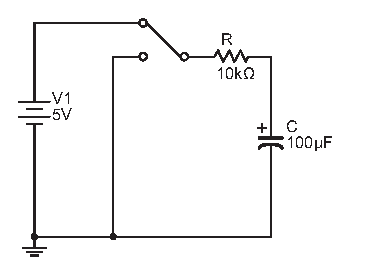
\includegraphics{capacitors/single_dc_capacitor.eps}
\hspace{0.5in}
\raisebox{0.2in}{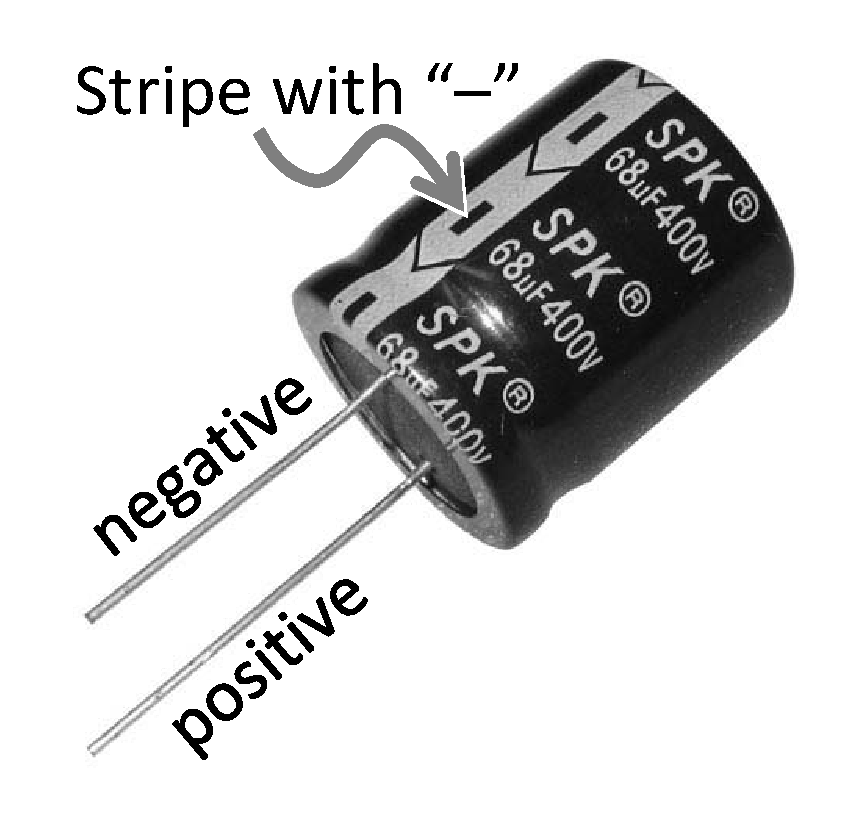
\includegraphics[height=1.3in]{capacitors/capacitor2_bw.eps}}
\end{center}

\item Examine the graphs you have just drawn, and predict where on the graphs the current is a maximum, and where it is a minimum.  Now insert your DMM as a current meter between $R$ and $C$, and test your prediction.  Were you correct?

\item When your capacitor is fully charged, throw the switch to discharge it, and measure the time it takes for $V_C$ to drop to about 1/3 of its original value (that is, from 5~V down to about 1.7~V).  This is called the ``time constant'' $\tau$ for this circuit.\footnote{More precisely, $\tau$ is the time for the voltage to fall to $1/e$ of its original value, where $e \approx 2.71828$.}

\item Make a prediction: if you increase the value of $R$, will the time constant increase or decrease?  Write your prediction first, then test it out.

\item Make another prediction: if you increase the value of $C$, will the time constant increase or decrease?  Again, write your prediction first, then test it out.

\item Now that you have several values of $R$, $C$, and $\tau$, care to hazard a guess about an equation relating those three?

\item Make a circuit like the one above with a time constant of 100 microseconds.   To verify the time constant with your oscilloscope, you will need to mess with the triggering for your scopes, so that the scope triggers only once as soon as you throw the switch, and doesn't trigger again.  You will need to change the trigger mode from ``auto'' to ``normal.''  (Look in your manuals.  What do these two modes mean?)

\item You have now seen the behavior of $V_C$ as a function of time for a discharging and charging capacitor.  Can you guess the functional form of $V_C(t)$ in each case?

\pagebreak[4]
\item The circuit below is similar to the Schmitt trigger you made in a previous lab, but instead of an arbitrary $V_{in}$, the negative input of the comparator is connected to $C_1$ and $R_5$.  
For the component values shown, what is the voltage at the $V_+$ input if $V_{out}$ is 0 volts?  
What is the voltage at $V_+$ if $V_{out}$ is 5 volts?  
If the switch is moved from $V_{CC}$ to ground, how long should it take $V_{out}$ to change?  How about when the switch is moved the other way?  Test this circuit, using your oscilloscope to measure the time delay between changes in $V_{in}$ and $V_{out}$. \label{part_delay_switch}

\begin{flushright}
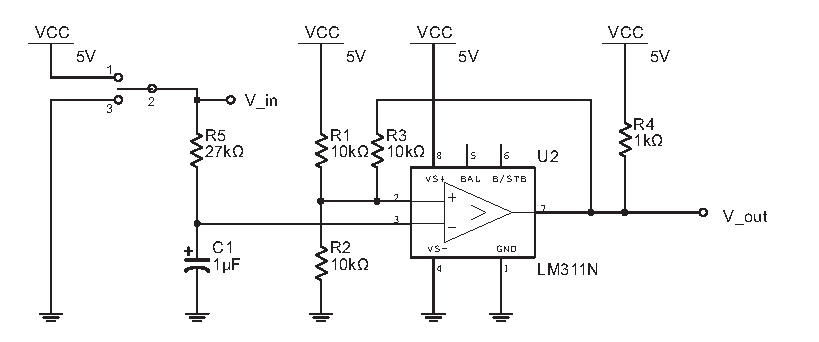
\includegraphics{capacitors/delay.eps}\hspace*{0.9in}
\end{flushright}

\item Modify the circuit slightly, replacing the switch with feedback from the output as shown below.   Draw three graphs of $V_+$, $V_-$, and $V_{out}$, all versus time, showing how they are synchronized with each other. \label{part_square_generator}
 
\begin{flushright}
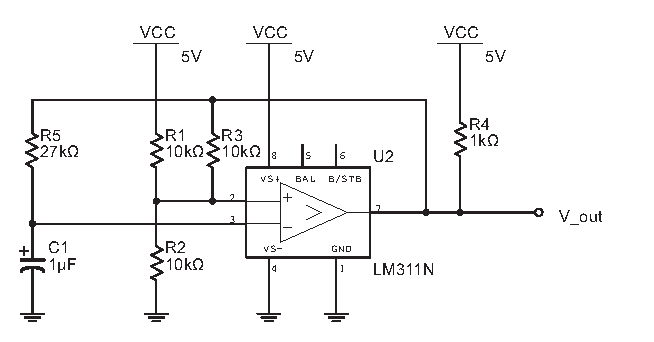
\includegraphics{capacitors/comparator_square_generator.eps}\hspace*{0.9in}
\end{flushright}

\item What capacitors and resistors can you change in order to increase the frequency of the output of the oscillator above?  What's the fastest output you can reasonably produce with this circuit?  Does it still look like a pretty square wave?  Which component of your circuit is the limiting factor in the speed of the output?
\end{enumerate}

\textbf{Possible Exam Questions:}

\begin{itemize}

%\item A 200~nF capacitor charges through a 2~k$\Omega$ resistor, starting at zero volts.  Graph both the current through the capacitor and voltage across the capacitor as a function of time.  At what time does the capacitor voltage reach 90\% of the supply voltage?  

\item For the circuit you built in part~\ref{part_rc_circuit}, draw graphs of $I(t)$ and $V_C(t)$ both while the capacitor is charging, and while it is discharging.  Also write equations for $I(t)$ and $V_C(t)$ for both charging and discharging.

\item What do ``Auto'' and ``Normal'' triggering modes mean on your oscilloscope?

\item For the circuit drawn in part \ref{part_square_generator}, graph voltage vs. time for the output terminal and each of the input terminals of the comparator.

%\item For the circuit drawn in part \ref{part_square_generator}, suppose $R_1=R_2=22$~k$\Omega$, $R_3=33$~k$\Omega$, $R_5=47$~k$\Omega$, and $C_1=2.2$~nF.  Calculate the output frequency of the oscillator.  For this problem, you may assume $R_4 \approx 0$. 

\item Use an LM311N comparator, as well as any other passive components you need (resistors, capacitors, etc.), to design a square wave generator with a frequency of about 150~kHz.  (Yes, on an exam you may be asked to design one of these from scratch, without a circuit diagram to guide you.)

\end{itemize}






\